\chapter{Overview of \gls{FFJ} and \gls{FFJ+}}\label{chap:offj}

\gls{FFJ} is a core calculus for \gls{FOP}, which was built 
upon an extension of \gls{FJ}---a minimal subset of Java. 
In \gls{FFJ}, classes can be added and modified by the 
introduction of a new feature, that is, 
an existing class can be extended by a class refinement. 
A class refinement is declared like a conventional class, though 
preceded by the keyword \texttt{refines}. For example, 
\texttt{refines class C \{$\dots$\}} refers to a class
refinement that
\emph{refines} the class \texttt{C}. The same can be achieved 
for method introduction and modification. Methods refinement,
however, override a previous definition of the corresponding 
method.
 
% \gls{FJ} models a minimal subset of Java. \gls{FFJ} extends \gls{FJ} for \gls{FOP}.
To fully mechanize \gls{FFJ}, we had to disambiguate and enhance 
the language to some extent that it  deserves the attention of 
formally documenting these changes. 
Even though these changes are significant, as discussed in \cref{chap:ffj}, 
the philosophy of \gls{FFJ}, \gls{FOP}, and Stepwise Refinement are maintained.
In \gls{FFJ}, as well as in \gls{FFJ+}, classes can be added and 
modified by the introduction of a new feature.
An existing class can be extended by a class refinement. A class refinement is declared like a class but
preceded by the keyword \texttt{refines}. For example, \texttt{refines class C@feat \{$\dots$\}} refers to a class refinement that
refines the class \texttt{C}. This way, a refinement may add new fields, and methods to the class
and override existing methods.  

A syntactical difference between \gls{FFJ} and \gls{FFJ+} is that, in \gls{FFJ+}, 
the feature notion appears in the abstract syntax tree (AST) of the language.
While the designers of \gls{FFJ} argue that the programmer does not have 
to explicitly state which feature a class or method belongs to, 
we favored the approach of stating the feature in the name of every refinement.
This greatly simplifies the structure of the formalism of the language and can be 
seen as an information gathered by the parser to build the AST, and thus 
the actual code expressed using the concrete syntax of this language 
might not have these annotations.

In addition, an \gls{FFJ+} program has a table with every class 
declaration (\textsf{CT}) and another table with every class refinement (\textsf{RT}).
We make this distinction to simplify the extension from \gls{FJ} in \texttt{Coq}, since 
with this decision we eliminate the need to match whether a class in the table 
is a refination or a declaration. From this \textsf{RT} we can retrieve the composition order
of the refinements and build the refinement chain of the program, 
which is used to check if features were composed correctly and
does not references features that have not been introduced yet. 
We redefine the denotation of \textsf{RT} from \gls{FFJ}.
In the original version, it was used to retrieve the refinement name given a 
refinement declaration. This is no longer necessary in \gls{FFJ+}, since
that information is already encoded in the abstract syntax.

Finally, in the original definition of \gls{FFJ}, the lookup functions are 
somewhat circumvoluted. Accordingly, we propose a very different approach
for them, with the aim as been not only as formal and simple as possible, 
but also easy to evolve from our mechanized version of \gls{FJ}. 
To this end, we eliminate the need for reverse field lookup, reverse method lookup, 
and the refinement relation. A formal description with all these changes 
is given in Section~\ref{subsec:lookup}. Note that, we were only 
able to conceive these improvements while formalizing \gls{FFJ+} in 
\texttt{Coq}. 

In \Cref{lst:expr-ct,lst:expr-rt} we revisit the EPL example from 
\Cref{seq:fop-ex} this time using \gls{FFJ+} instead of AHEAD.

\begin{lstlisting}[language=Java, frame=single, numbers=left, basicstyle=\footnotesize,
    label={lst:expr-ct}, caption={EPL Class Table}, captionpos=b]
class Expr extends Object {
    Expr() { super(); }
}

class Add extends Expr {
    Expr a; Expr b;
    Add(Expr a, Expr b) {super(); this.a=a; this.b=b;}
}

class Sub extends Expr {
    Expr a; Expr b;
    Sub(Expr a, Expr b) {super(); this.a=a; this.b=b;}
}
\end{lstlisting}

\begin{lstlisting}[language=Java, frame=single, numbers=left, basicstyle=\footnotesize,
    label={lst:expr-rt}, caption={EPL Refinement Table}, captionpos=b]
refines class Expr@Eval {
    refines Expr() { original(); }
    int eval() {return 0;}
}

refines class Add@Eval {
    refines Add(Expr a, Expr b){original(a,b);}
    refines int eval() {return this.a.eval() + this.b.eval();}
}


refines class Sub@Eval {
    refines Add(Expr a, Expr b){original(a,b);}
    refines int eval() {return this.a.eval() - this.b.eval();}
}
\end{lstlisting}

Typically, a programmer applies multiple refinements to a class by composing
a sequence of features. The ordered list of refinements is called a \emph{refinement
chain}. The order in which a refinement introduced matters, and a refinement
that is introduced right before another is called \emph{predecessor}. 

As class inheritance, refinements cannot introduce a field with the same
name already declared before. Methods, on the other hand, may overload an already
introduced class, this can be seen in \texttt{Sub@Eval eval} and \texttt{Add@Eval eval}.
Overloading, on the other hand, is not allowed, i.e. if the programmer wants to introduce the
a method with a name that is already used, it must have the same number of arguments, the same argument types
and the same return type as the previous function definition.

The distinction between method introduction and overriding allows the type system to check
if an introduced method inadvertently replaces an existing one with the same name.
The distinction also allows the type system to check if there is proper a method to be overridden.

In order to retrieve the correct fields or the correct method of a class, it is
necessarily to walk in the subclass refinement correctly. As shown in \Cref{fig:refinement-order}
first start from the last refinement of a class, walk through every predecessor,
and when you get to the last refinement, you go to the class, and finally to the
superclass last refinement. And so on until you reach the Object class, which
is the root class of all class hierarchies.

\begin{figure}[htb]
    \centering
    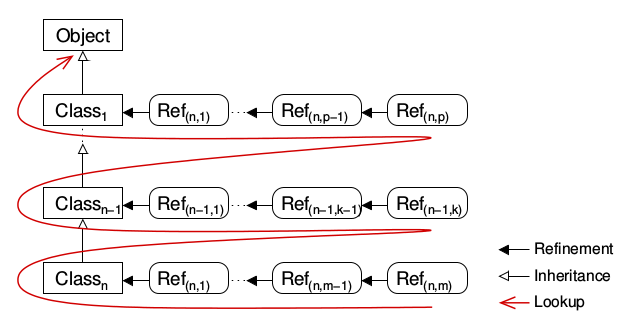
\includegraphics[scale=0.7]{doc/images/refinement-order}
    \label{fig:refinement-order}
    \caption{Order of lookup in \gls{FFJ+}}
\end{figure} 

